\section{Experimental Evaluation}\label{sec:evaluation}

\begin{table}
\centering
\begin{tabular}{|l|r|r|r|r|}
\hline
\bf{Dataset}&\bf{Size}&$\sharp$\bf{Col}&\bf{Value types}&\bf{Max rows}\\
\hline
Routing&5.4G&4&\small{int, long}&240M\\
SDSS&6.2G&4008&\small{real, double, long}&47M\\
Cnet&12G&2991&\small{int, char}&1M\\
Airtraffic&29G&93&\small{int, short, char, str}&126M\\
TPC-H 100&168G&61&\small{int, date, str}&600M\\
\hline
\end{tabular}
\caption{Dataset statistics.}
\label{tbl:dataset}
\end{table}

We performed an extensive experimental study to gain insights into the
applicability of the imprints index, the storage overhead and creation
time, as well as the query performance. We compare our index with two
state-of-the-art commonly used secondary index solutions, namely \it{zonemaps}
and \it{bit-binning} with \it{WAH encoding}. We also provide, for a baseline
comparison, the time measurements for sequential scan. In order to study the
impacts of different value types, different column sizes, and different value
distributions, we used real world datasets gathered from various test cases.
These datasets are either publicly available or part of in-house projects.

\begin{figure*}[t]
\centering
\tabcolsep2pt
\begin{tabular}{m{4cm}|m{4cm}|m{2.2cm}|m{2cm}|m{4cm}}
{%
\fontsize{3}{0}%
\selectfont%
\begin{verbatim}......................x.xx...xx..xx.x..x...xx...x..x..x.x.......
.....x..xx.xx.....x...xx...x........xx.................x...xx...
.................................x..xx......x...x...x.x.x.xxx...
..................x....x.x.x.x....xx..x.x.x.x...x..x..x.x.......
........x.xxx...xx...xx.x..x....x.x..x........x........x........
......x.......................x.......x.....xxx.x..xxx..xxxx....
.........x..xxx...x...x.x.xx.....x.....x....x..x....x...........
...x.....x..xx............x.............x.x....x.xx..xxx........
.......x..x......x....x..x......x.x..xx.....x.....x..x..........
.xx.x..xxx..x....xx.x....x...x.............x.x.x................
.x.xx.....x..x....x...x....x.xx....x.xxx........................
..x.x......x.x.....x.x..........x.x................xx.....xxx...
............................x...x.....x.x.x.x.xx....x.x.x.xx....
..x.......x.x..xxxxx..xx..x...x..x................x.............
..........................................xxx......x.xx..xxxx...
........x.....x.......x.x.......x...xx..x...x.....x.x.x.xxx.....
..x..x.x.xx.x...xx.xx.............x....................x....x...
...................................x..x...x.x.....xx..x.xxxxxx..
.......x.x.....x...x........xx..x.x....x...x......xx....x...x...
.................................x......xx.x......x...x.xx.xxx..
.....x..xx...x.x.x...x......xx..xx.....x.x.......x........x.....
.x.....x...x....................x...xxxxxxxx.x..x.....x.........
......x..x.x.x..x.x......x....xx..x.xx...................x......
.......................x................x.x..x.x....x..xxxxxx...
....xxxx.....x..x.x.x..x...xx.....x.............x..x.x...x......
...........................................xx.....xx..x.x.xxx...
................x......x.......xxx........x..x...xx.x.x..xx.....
............xx.....x..x.xxx.xx..x..................x.....x.xx...
.........................x..................x....x.x..x.xxxxx...
......x.......x.....x.x.x...xxx........x.x.x...xx...xx..........
.....x......xx...xx..x....xxx.........x.......x..........xx.....
.............x......x.....x.....xx..x..x.xx.x....x...xxxxx......
............xx..x...xx....x.x...xx.........xx......x....x.......
..........................x....xx.x..x...x.xx.xx..xx..x.........
.x........x..xx.x..xx..x...x....xx.....................x...x....
............x...................x..xx.........xx....xx.x..xxx...
.......x.xxx......x..xx.x.xx..x.x......x...x..........x.........
............x..................x.......x.....x.......x.x.xxxx...
............x.........xxx.....x....xx.....xx...x..x..x..xx......
....x......xx.....xxx..x.x...................x......x.....xx....
.........x.......x............x....x.x...x.....x..x.xx..xxxx....
........xx...xx.....xx.......x.....xx..x.......x...x....x..x....
....................................x.x.......x...x..xxx.xxxx...
..................xx..x.......x.x..x.x.x..x.....x..x.x....x.....
....x....x......x............x.............x.x..x...x...xx..x...
....x.x.x.......x.x.........x.x...x..x..xx.........x.....xxx....
.......x...xxx.xxx...x..........xxx.x..............x....x...x...
......x................................x.xx.....xxx..x..xx.xx...
.....xx...x..xx..xx.....x...x..x.x.............x...x.....x......
..................x..........x.......x...x.x.x.xx...x...x.xxx...
......xx.xx...xx..xx.....x.xxx..x..x..x..........x..............
.x......................x......xx..x........xx...x...xx.x..xx...
.x...xx..x..xx......xx.x........x....x...........x......x.......
..................x..x.......x.....x......x......x..x...xxxxx...
......x...x.x....x.x...xxx.....x....x.x....x....x....x..........
......x..........................x.x..........xx.x..x...xxxxx...
.....x....................x........xx...x.x..x..x...x..x.x.x....
.x...x..x.....x...x....xx.x.xx..................x...x.....x.x...
...................x......x..x..........xx.......x.x.x.xx.xxx...
.........x.xxxxx......xx.....x..xx...xx..xx.....................
.x.x.xx.............x....................x.....x....x..x.x.xx...
..xx......xx.xx...xx.x.........x.x.x....x.........x...x....x....
.....x.x................x.......x.........x......x..x..xx.xxx...
.x....x.x..x.....xxx.x..x.......x..x.....x.x........x.x.........
...x....x.................................x.x.x....xxx...xxxxx..
..x..xx..x.x.............x.x.x.x.....x......xx........x..x......
.xx..........x.............x........x.....x..xx..x....xx.x.xx...
...x....x...x...x..x...xx.....xx...x..xx...........x....x..x....
....x..x.................x...............xx.....x..xx..x.x.xx...
..x.x...x...x..........x.x..x....xx...x....x.......x..x....x....
............xxx..x.....x.xx..xx......x...x......................
..x..x..........................x.........x.....x..xx..x.x.xx...
....x.x...x.....xx..x...x.x.x.....x...x....x.......x..x.........
........x...x.x....xx.x..xx................x....x....x...x......\end{verbatim}
}
&{%
\fontsize{3}{0}%
\selectfont%
\begin{verbatim}..x.............................................................
..xx............................................................
..x.x...........................................................
..xxx...........................................................
...xx...........................................................
....x...........................................................
....xx..........................................................
.....x..........................................................
.....xx.........................................................
......x.........................................................
......x..x......................................................
......x.xx......................................................
......x.xxx.....................................................
......x.x.x.....................................................
......xxx.xx....................................................
.......x..xx....................................................
......xx..xx....................................................
.......x...x....................................................
......xx...xx...................................................
......xx....x...................................................
.......x....x...................................................
............x...................................................
............x.x.................................................
.............xx.................................................
..............x.......................x.........................
......................................x.........................
.....................................x..........................
.....................................x................x.........
......................................................x.........
.....................................................xx.........
.....................................................x..........
..................................................x..x..........
..................................................x.............
.................................................xx.............
.................................................x..............
.........x.......................................x..............
.........xx.....................................................
..........x.....................................................
.........xx.....................................................
.........x......................................................
........xx......................................................
........x.......................................................
.......xx.......................................................
.......x........................................................
.......x..x.....................................................
..........x.....................................................
.........xx.....................................................
.........x......................................................
.........x............................x.........................
......................................x.........................
......................................xx........................
......................................x.........................
.....................................x..........................
....................................xx..........................
....................................x...........................
...................................xx...........................
...................................x............................
...................................xx...........................
....................................x...........................
...................................x............................
................x..................x............................
................x...............................................
................xx..............................................
.................x..............................................
.................xx.............................................
..................x.............................................
..................xx............................................
...................x............................................
....................x...........................................
....................xx..........................................
.....................x..........................................
.................x...x..........................................
.....................x..........................................
.....................xx.........................................\end{verbatim}
}
&{%
\fontsize{3}{0}%
\selectfont%
\begin{verbatim}.x..............................
.xx.............................
..x.............................
..xx............................
...x............................
...xx...........................
....x...........................
....xx..........................
.....x..........................
.....xx.........................
......x.........................
......xx........................
.......x........................
.......xx.......................
........x.......................
........xx......................
.........x......................
.x.......x......................
.x..............................
.x........x.....................
..........x.....................
..........xx....................
...........x....................
......x....x....................
......x.........................
......x.....x...................
............x...................
............xx..................
.............x..................
.............xx.................
..............x.................
..........x...x.................
..........x.....................
.x........x.....................
.x..............................
.xx.............................
..x.............................
..xx............................
...x............................
...xx...........................
....x...........................
.....x..........................
.....xx.........................
......x.........................
......xx........................
.......x........................
.......xx.......................
........x.......................
........xx......................
.........x......................
.x.......x......................
.x..............................
.x........x.....................
..........x.....................
..........xx....................
...........x....................
......x....x....................
......x.........................
......x.....x...................
............x...................
............xx..................
.............x..................
.............xx.................
..............x.................
..........x...x.................
..........x.....................
.x........x.....................
.x..............................
.xx.............................
..x.............................
..xx............................
...x............................
...xx...........................
....x...........................\end{verbatim}
}
&{%
\fontsize{3}{0}%
\selectfont%
\begin{verbatim}......xx........
......xxx.......
......xx........
......xxx.......
......xx........
x.....xx........
......xx........
x.....xx........
......xx........
x.....xx........
......xx........
x.....xx........
......xx........
x.....xx........
......xx........
x.....xx........
......xx........
x.....xx........
x.....xx........
......xx........
x.....xx........
......xx........
x.....xx........
......xx........
.x....xx........
......xx........
.x....xx........
......xx........
.x....xx........
......xx........
.x....xx........
......xx........
.x....xx........
......xx........
.x....xx........
......xx........
.x....xx........
......xx........
.x....xx........
......xx........
..x...xx........
......xx........
..x...xx........
......xx........
..x...xx........
......xx........
..x...xx........
..x...xx........
......xx........
..x...xx........
......xx........
..x...xx........
......xx........
..x...xx........
......xx........
..x...xx........
......xx........
...x..xx........
......xx........
...x..xx........
......xx........
...x..xx........
......xx........
...x..xx........
......xx........
...x..xx........
......xx........
...x..xx........
......xx........
...x..xx........
......xx........
...x..xx........
......xx........
...x..xx........\end{verbatim}
}
&{%
\fontsize{3}{0}%
\selectfont%
\begin{verbatim}.x...................................x..........................
.x...................................xx.........................
.x....................................xx........................
.x.....................................x........................
.x.....................................xx.......................
.x......................................x.......................
.x......................................xx......................
.x.......................................x......................
.x.......................................xx.....................
.x........................................x.....................
.x........................................xx....................
.x.........................................x....................
.x.........................................xx...................
.x..........................................x...................
.x...........................................x..................
.x...........................................xx.................
.x............................................xx................
.x.............................................x................
.x.............................................xx...............
.x..............................................xx..............
.x...............................................x..............
.x...............................................xx.............
.x................................................x.............
.x................................................xx............
.x.................................................x............
.x.................................................xx...........
.x..................................................x...........
.x..................................................xx..........
.x...................................................x..........
.x...................................................xx.........
.x....................................................x.........
.x....................................................xx........
.x.....................................................x........
.x.....................................................xx.......
.x......................................................xx......
.x.......................................................x......
.x.......................................................xx.....
.x........................................................x.....
.x........................................................xx....
.x.........................................................x....
.x.........................................................xx...
.x..........................................................x...
.x..........................................................xx..
.x...........................................................x..
.x...........................................................xx.
.x............................................................x.
.x............................................................xx
.x.............................................................x
.x.....x.......................................................x
.x.....x........................................................
.x.....xx.......................................................
.x......x.......................................................
.x......xx......................................................
.x.......x......................................................
.x.......xx.....................................................
.x........xx....................................................
.x.........x....................................................
.x..........x...................................................
.x..........xx..................................................
.x...........x..................................................
.x...........xx.................................................
.x............x.................................................
.x............xx................................................
.x.............xx...............................................
.x..............x...............................................
.x..............xx..............................................
.x...............x..............................................
.x...............xx.............................................
.x................x.............................................
.x................xx............................................
.x.................x............................................
.x.................xx...........................................
.x..................x...........................................
.x..................xx..........................................\end{verbatim}
}
\\
\hline
SDSS&Routing&Airtraffic&Cnet&TPC-H 100\\
 \it{photoprofile.profmean}&\it{trips.lat}&\it{ontime.AirlineID}&\it{cnet.attr18}&\it{part.p\_retailprice}\\
$\mathcal{E}=0.794214$&$\mathcal{E}=0.312631$&$\mathcal{E}=0.351838$&$\mathcal{E}=0.200114$&$\mathcal{E}=0.228922$\\
%\hline
\end{tabular}
\caption{Prints of column imprint indexes (\tt{'x'} = bit set, \tt{'.'} = bit unset) and the respective column entropy $\mathcal{E}$.}
\label{fig:snap}
\end{figure*}

Column imprints, zonemaps, and WAH are all implemented in C, and the code
is available for review upon request.%In addition, imprints will be part of
%a future release of MonetDB.
The implementation of zonemaps and WAH follow the
same coding style and rules as imprints to ensure fairness of comparison.
Each experimental run is done by first copying a column into main memory, and
then creating the zonemap, imprints and WAH indexes. The timer is always
started during the snippets of code that implement each index, thus avoiding
measuring administrative overhead, which may not be common for all indexes. We
report the wall-clock time as returned by the timing facilities of the
\tt{time.h} library of C. All code has been compiled with the \it{clang}
compiler with optimization level 3.

Zonemaps are implemented as two arrays containing the min and max values of
each zone. The size of the zones is chosen to be equal to the size that each
imprint vector covers, i.e., the size of the cacheline. The min and max
arrays are aligned with the zone numbering, i.e., the first min and max values
correspond to the minimum and maximum values found in the first zone, and so
on. For the bit-binning approach of bitmaps, the bins used are identical to
those used for the imprints index, as described in the \tt{binning()} procedure
of Algorithm~\ref{alg:binning}. Using this binning scheme, each value of the
column sets the appropriate bit on a vector large enough to hold all records. To
compress the resulting bit-vectors we apply WAH compression with word size
32 bits, as described in~\cite{WOS02}.

All experiments were conducted on an Intel\textsuperscript{R}
Core\textsuperscript{TM} i7-2600 cpu @ 3.40GHz machine with 8 cores and 8192 KB
cache size. The available main memory was 16 GB, while the secondary storage
was provided by a Seagate\textsuperscript{R} Constellation\textsuperscript{TM}
SATA 1-TB hard drive and capable of reading data with a rate of 140MB/sec.

%\subsection{Data Analysis}
%
%We begin the presentation of our experimental analysis by first describing in
%detail the datasets used. We then introduce a novel metric, called
%\it{column entropy}, to quantify the clustering property of the values of a
%column.
%
\begin{figure}
\includegraphics{figs/static/cumul}
\caption{Cumulative distribution of the columns' entropy $\mathcal{E}$.}
\label{fig:cumentr}
\end{figure}

\begin{figure*}[t]
\centering
\tabcolsep2pt
\begin{tabular}{cccc}
\includegraphics{figs/static/storage_rpp64}&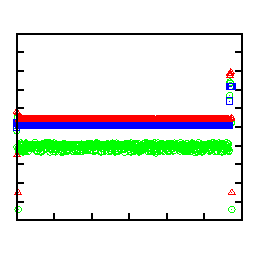
\includegraphics{figs/static/storage_rpp32}&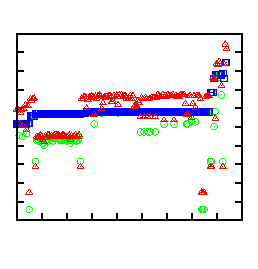
\includegraphics{figs/static/storage_rpp16}&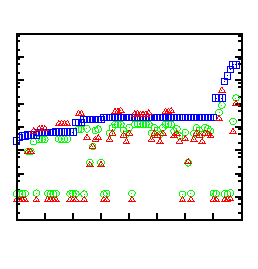
\includegraphics{figs/static/storage_rpp8}\vspace{-15pt}\\
\includegraphics{figs/static/storagetime_rpp64}&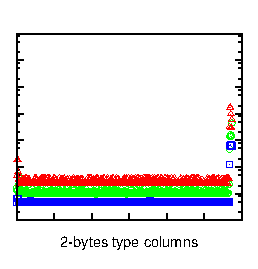
\includegraphics{figs/static/storagetime_rpp32}&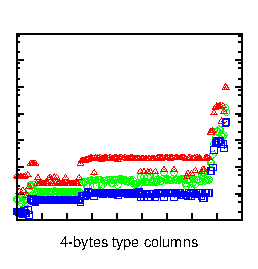
\includegraphics{figs/static/storagetime_rpp16}&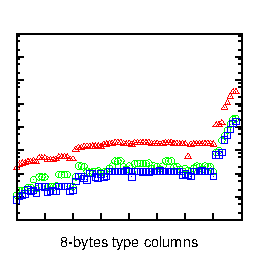
\includegraphics{figs/static/storagetime_rpp8}
\end{tabular}
\caption{Index size and creation time for different types of columns ($x$-axis enumerates the columns, ordered by size).}
\label{fig:storage}
\end{figure*}

Table~\ref{tbl:dataset} lists the name, the size in gigabytes, the total number
of columns, the column types, and the maximum number of rows of the datasets
used for our experimentation. The first dataset, denoted as Routing, is a
collection of over 240 million geographical records (i.e., longitude, latitude,
trip-id, and timestamp) of ``trips'' as logged by gps devices. The next
dataset, SDSS, is a 6.2 GB sample of the astronomy database
SkyServer. This database contains
scientific data, with many double precision and floating point columns
following a uniform distribution, thus stressing compression techniques to their
limits. Cnet is a categorical dataset describing the properties of technological
products. All data are stored on a single but very wide table, where each
column is very sparse, thus presenting ample opportunities for
compression. The dataset was re-created based on the study of
J.Beckham~\cite{cnet}. The Airtraffic delay database represents an ever growing data warehouse with statistics about flight
delays, landing times, and other flight statistics. The data are updated per
month, leading to many time-ordered clustered sequences. Lastly, we used the
TPC-H benchmark dataset with scale factor 100, in order to
compare against a well recognizable dataset.

\subsection{Column Entropy}

We wish to better study the properties of the columns that are typically not
ordered, part of very wide tables, and eligible for secondary indexing. Our
initial motivation was based on the observation that ``secondary data'' exhibit
some degree of clustering, either inherited during the creation process of the
data, or indirectly imposed by the few columns that are ordered because of
primary indexing. Column imprints are designed such that this clustering is
naturally exploited without the need of explicit configuration. This is why
imprints are built per block and compressed row-wise per imprint vector,
instead of vertically per bin.
To better understand and quantify the degree of clustering found in data, we
define a new metric, called \it{column entropy}. Column entropy measures how close
a column is to being ordered, or, in other words, the amount of clustering found
in a column when the values are partitioned into bins. More formally, column
entropy $\mathcal{E}$ is defined to be
$$\mathcal{E}=\frac{\sum^{n}_{i=2}d(i,i-1)}{2\times\sum^{n}_{i=1}b(i)}$$
where $d(i,i-1)$ is the \it{edit distance} between bit-vector $i$ and $i-1$,
and $b(i)$ is the number of bits that are set in bit-vector $i$. We define the
edit distance between two bit-vectors to be the number of bits that need to be
set and unset in the first bit-vector in order to become the second. Column
entropy $\mathcal{E}$ takes values between $0.0$ and $1.0$. The higher the
entropy $\mathcal{E}$ the more random the data is and the less clustered it
appears to be.

To give a more intuitive view of \it{column entropy}, we print a
small portion of the column imprint index of five columns, one from each
dataset, and list them in Figure~\ref{fig:snap}, together with their respective
entropy value $\mathcal{E}$. The prints in Figure~\ref{fig:snap} correspond to
the actual imprint indexes as constructed in our code for the experiments. If a
bit is set then an \tt{`x'} is printed, otherwise an \tt{`.'}. The first
column imprint of Figure~\ref{fig:snap} corresponds to a column from the
SkyServer dataset. It is of type real and has a high entropy value of almost
$0.8$ which implies that each next imprint vector is significantly different
from the previous one. Such columns with high entropy, as demonstrated in the
next section, are harder to compress. The next imprint is the latitude
attribute of the Routing dataset. It exhibits nice clustering properties,
something to be expected since the dataset is taken from real observations, and
thus trips are continuous without any jumps, unless the trip-id changes. The
next two imprints are taken from the Airtraffic and Cnet dataset. These are
categorical datasets, with low cardinality -- hence the smaller bit-vectors --
and with low entropy value. The last imprint index is the \it{retail\_price}
attribute of table \it{part} of TPC-H. This dataset is created to contain a
sequence of prices that are not ordered, but they are still the same repeated
permutation of an order. Such an organization of data resembles closely an
ordered column, and thus also has a low entropy value.

Figure~\ref{fig:cumentr} depicts the cumulative distribution of the entropy
$\mathcal{E}$ for all columns of all datasets that we used in our experiments.
We exclude all columns that are less than $1$ megabyte in size, since
they are of minimal interest and introduce outliers in our measurements. More
than $3000$ columns have entropy smaller than $0.4$, thus supporting our claim
that data often tend to exhibit good local clustering and ordering properties.
Nevertheless, there are almost a thousand columns that have high entropy
values, up to almost $1.0$. Those columns are not to be ignored since they sum
up to over $20$\% of the total data. A secondary index should be immune to such
high entropy, and still be able to take advantage of any opportunities for
compression. In the next section we study the storage overhead of imprints and
other state-of-the-art secondary indexes, while giving emphasis to their
behavior on columns with high entropy. We show that imprints are robust
against columns with high entropy, while bitmaps with WAH fail to achieve a
good compression rate.

\subsection{Index Size and Creation Time}

We analyze the storage overhead introduced by the column imprints index
and compare it with that of zonemaps and WAH. The upper row of the graphs in
Figure~\ref{fig:storage} depict the sizes of the indexes over all columns and
all datasets. Each graph corresponds to a different value type. For
presentation reasons, we divide the types according to their size in bytes. For
example, char is $1$-byte, short is $2$-byte, int and date are
$4$-byte, and long and double $8$-byte types. The $y$-axis depicts the size of
the indexes measured in megabytes, starting from a few bytes for the smaller
columns to almost one gigabyte for the large ones. Notice that $y$-axis is
\it{log-scaled}. The $x$-axis orders the columns according to their size (in
increasing order). However, because many columns have exactly the same size,
since they originate from the same tables, we distinguish them by placing them
next to each other. As a result, the flat horizontal patterns appearing in the
graphs correspond to different columns of the same size, while the
``stepping'' effect corresponds to the next group of larger columns.

\begin{figure}
\includegraphics{figs/static/percentage}
\caption{Index size overhead \% over the size of the columns.}
\label{fig:perc}
\end{figure}

The red triangle points mark the size of the bit-binning index with WAH
compression, the blue squares mark the size of zone\-maps, and the green
circles mark the size of the column imprints index. The general
picture drawn for all types is that WAH index entails the largest storage
overhead, zonemaps come second, while imprints have the least
requirements of storage space. More specifically, the general trend is that
imprints are between one and two orders of magnitude more space efficient
than zonemaps and WAH. However, there are exceptions to that rule, especially
for WAH indexing, which depicts the biggest fluctuation in storage needs. For
$1$-byte types, there are cases where WAH achieves better compression and
reaches that of imprints. By examining the data closer we noticed that this is
true for columns that although they have more than 126 million rows (taken from
the Airtraffic dataset), they only contain two distinct values, thus allowing
both WAH and imprints to fully compress their bit-vectors. Another point of
interest is found in the case of $8$-byte types, where WAH can become a bit
more space efficient than imprints. This is true for those columns that contain
primary keys (e.g., bigint identifiers) and in addition are ordered.
Although we are studying secondary indexes that typically apply to unordered
columns, we did not exclude any ordered columns from our experimental datasets
for completeness.

Since it is impractical and hard to explicitly show the size of each individual
column, we compute the percentage of the size of the indexes over the size of
the column. Figure~\ref{fig:perc} shows such a graph. In addition, instead of
grouping on value type, we group columns from the same datasets together, such
that more insights about the different applications, and hence different value
distributions can be gained. The categorical data Cnet which has columns with
low cardinality, as well as the nicely clustered routing dataset, achieve the
best compression for both imprints and WAH, thus requiring in many cases
less than 10\% space overhead. However, the same can not be said for broader
value domains and uniform distributions. Specifically, the scientific
dataset of SkyServer, consisting of many columns with real and double values,
with high cardinality and no apparent clustering, makes the WAH index very
unstable and induces high storage overhead. Imprints perform fairly stably
and much better than WAH, with space overhead closer to zonemaps. The failure
of WAH is expected due to the high randomness of the values in SkyServer, which
allows for very few compression opportunities. However, imprints do not suffer
from the same problem. Since one imprint vector is constructed for each
cacheline, the space requirements are less than bitmaps, while the chance of
consecutive imprint vectors to be identical, and thus compressible, is
increased.

Figure~\ref{fig:entropy} depicts the index size overhead of both imprints
and WAH as percentage of the size of the column, ordered over the entropia
$\mathcal{E}$. Imprints achieve storage overhead less than 10\% for
columns with low entropy, i.e., up to $0.4$. The same observation holds with
few exceptions for WAH indexing. However, the picture changes for columns with
entropy of $0.5$ and higher. Imprints exhibit a steady storage overhead
that hardly exceeds 12\%. WAH indexing suffers more, with up to almost 100\% of
storage overhead on the size of the column. Imprints on the one hand need
at most 64 bits per cacheline unit, making them immune to high entropy,
while benefiting from low entropy. On the other hand, WAH can potentially
become very inefficient. If there are very few opportunities for compression,
most 32-bit words will be aligned with 31-bit literals, i.e., no big long
sequences of same bits will be found in the bit-vectors. In addition, since we
use a 64 bit-binning approach, there will potentially be 64 uncompressed bits
per value. All in all, WAH is more suitable for low entropy data, while
imprints are more stable and with better compression for the entire range of
entropy values, i.e., they work even if data are not locally clustered.

\begin{figure}
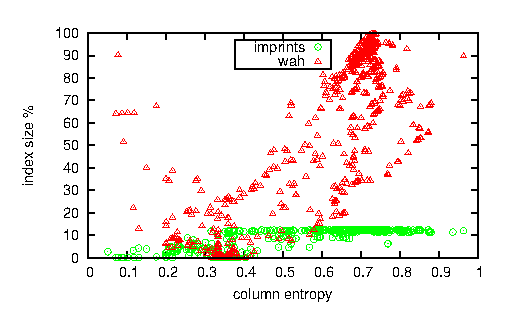
\includegraphics{figs/static/entropy}
\caption{Index size overhead \% over column entropy $\mathcal{E}$.}
\label{fig:entropy}
\end{figure}

Another concern is the time spent to create each secondary index. The bottom
row of graphs in Figure~\ref{fig:storage} depicts the creation time for WAH,
zonemaps, and imprints. As expected the zonemaps are the fastest to create.
For each row only two comparisons have to be made to determine the minimum
and the maximum values for the current zone. The slowest is the WAH index,
since there is significantly more work to be done in order to compress the
bit-vectors. Imprints on the other hand, always perform between zonemaps and
WAH. The overall differences of the construction time between the three indexes
is steady and to be expected since each of them require a different amount of
work per value. Most importantly, the time for all indexes increases linearly
to the size of the columns, thus making them a cost-effective solution for
secondary indexing.

\subsection{Query Performance}

Next, we turn our attention to the performance analysis of evaluating range
queries. The execution scenario for this set of experiments is as follows. For
each column, ten different range queries with varying selectivity are created.
The selectivity starts from less than $0.1$ and increases each time by
$0.1$, until it surpasses $0.9$. These 10 queries are then fired against the
three indexes (i.e., zonemaps, WAH, and imprints) defined over the column,
and also evaluated with a complete scan over that column. The result set of
each query is a materialized ordered list of \it{id}'s. The ordering of
\it{id}'s is guaranteed by the sequential scan, the zonemap index, and the
imprints index. However, this is not true for WAH, since each pass over the
different bit-vectors will produce a new set of \it{id}'s which needs to be
merged. The merging is done by defining another bit-vector aligned with the
\it{id}'s. The bits that are set in this \it{id} bit-vector correspond to the
\it{id}'s that satisfy the range query. In this way no final merge is needed,
just the materialization of the \it{id}'s. This implementation only adds a
small, but necessary for fairness, overhead to WAH compared to the other
indexes.

\begin{figure}
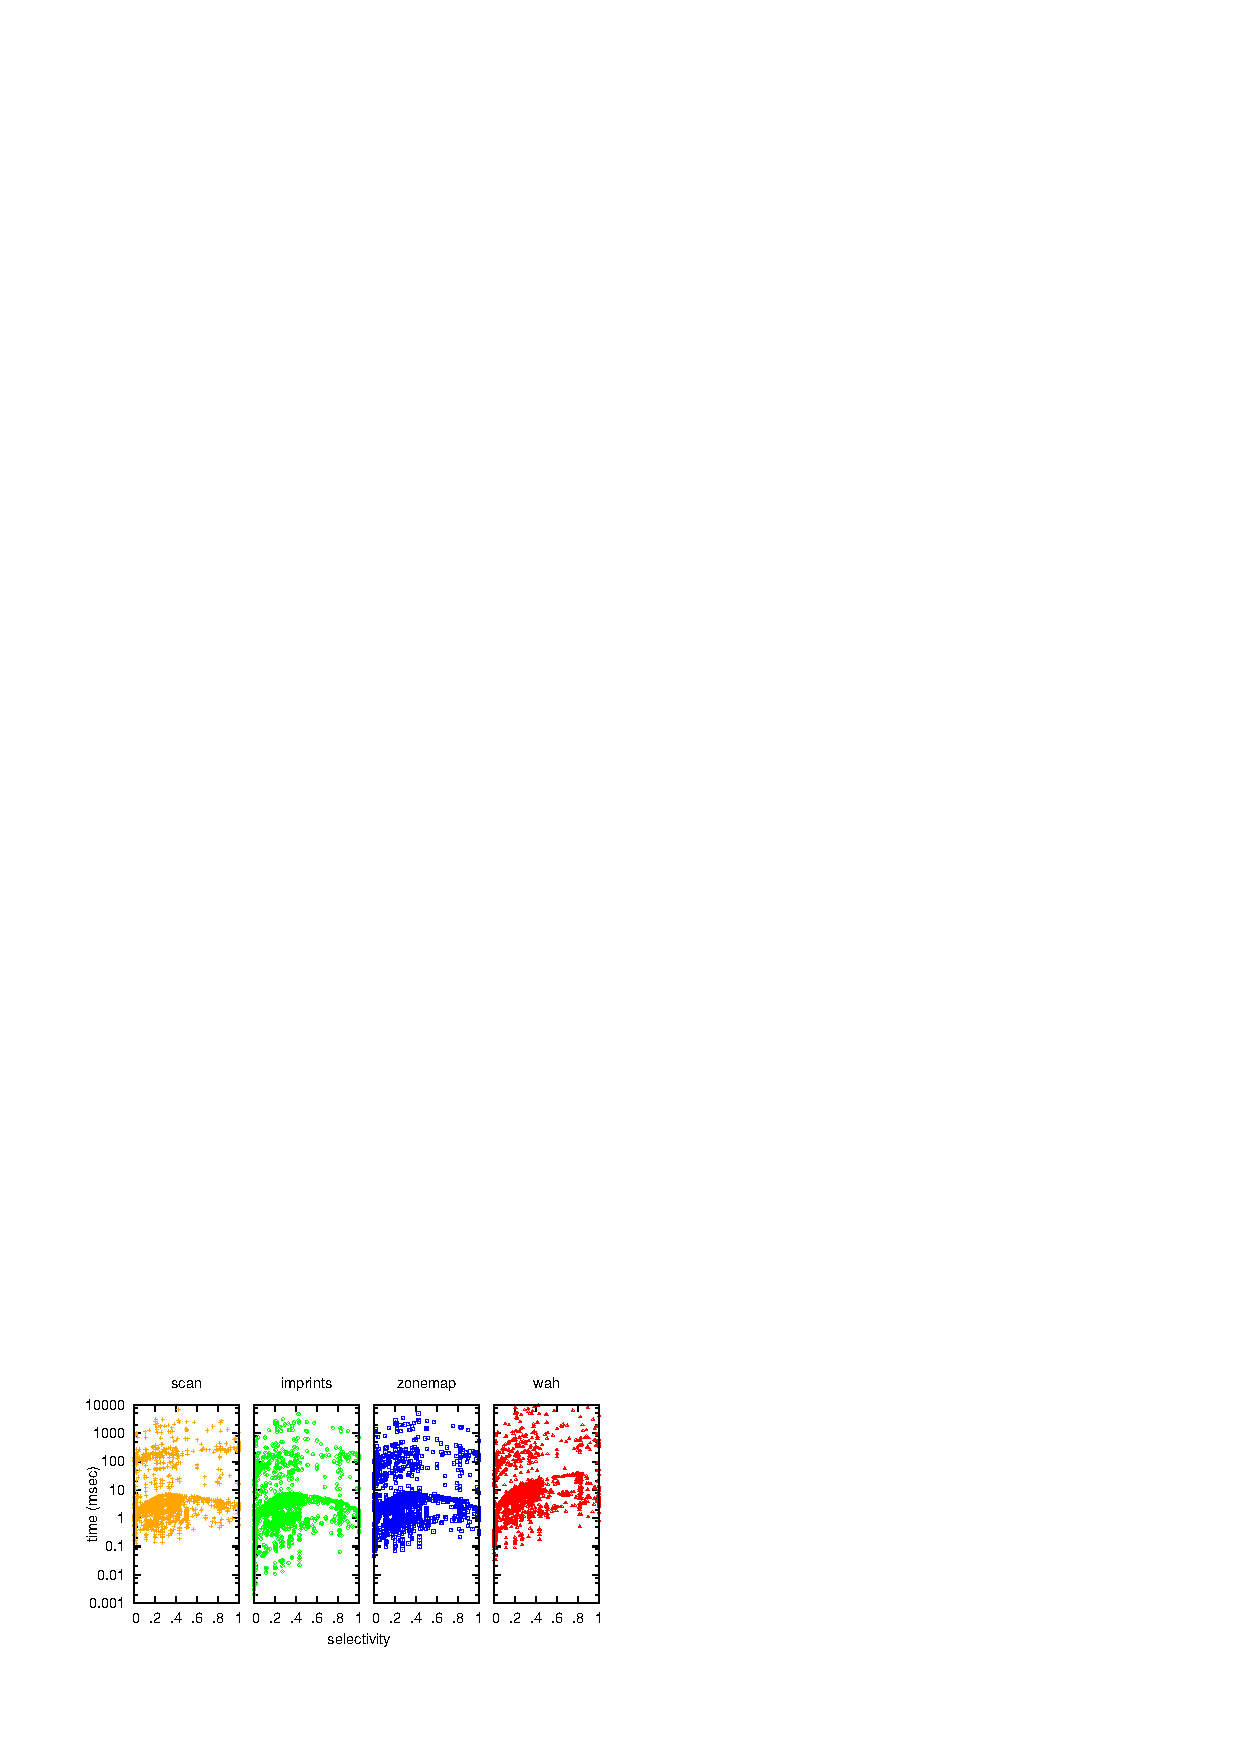
\includegraphics{figs/static/qtime}
\caption{Query time for decreasing selectivity.}
\label{fig:queryt}
\end{figure}

Figure~\ref{fig:queryt} plots the query times of over 40,000 queries evaluated
over each index. The queries are ordered on the $x$-axis according to their
selectivity. If the selectivity is $0.1$, the query returns 10\%
of the total values in the column, while $0.9$ returns 90\% of the total
values. All three indexes and the sequential scan produce the same graph
patterns for query times. However, these patterns are shifted along the
$y$-axis. Imprints is the fastest index overall since the points in the graph
are shifted the most to the bottom. As expected, if the selectivity of the
query is low and thus more data are returned, the smaller the differences that
are observed between indexes. In fact, sequential scans then also become
competitive. This is due to the fact that the overhead of decompressing
the data, and materializing almost all of the \it{id}'s,
surpasses the time needed to sequentially scan the entire column and check each
value. In addition, zonemaps exhibits query times similar to that of
sequential scan for low selectivity queries, since zonemaps require the least
administration overhead compared to imprints and bitmaps with WAH.

\begin{figure}
\includegraphics{figs/static/cum_queries}
\caption{Cumulative distribution of query times.}
\label{fig:queryc}
\end{figure}

To better understand the behavior of zonemap, WAH, and imprints, for
queries with high selectivity, and compare them with sequential scans, we
plot in Figure~\ref{fig:queryc} the cumulative distribution of the queries over
time. More precisely, we count the queries that finish execution at each time
frame, and cumulatively sum them up. The steeper the graph in
Figure~\ref{fig:queryc} the more queries finish in a shorter time, thus the
more efficient the index is overall. Figure~\ref{fig:queryc} shows that almost
$15,000$ queries need each of them less than $0.1$ milliseconds to be evaluated
with imprints index. Zonemaps, which is the second best, manage to evaluate
just over 7,500 queries in the same time frame. However, as the evaluation
time increases the time gap between the different approaches is reduced.

\begin{figure}
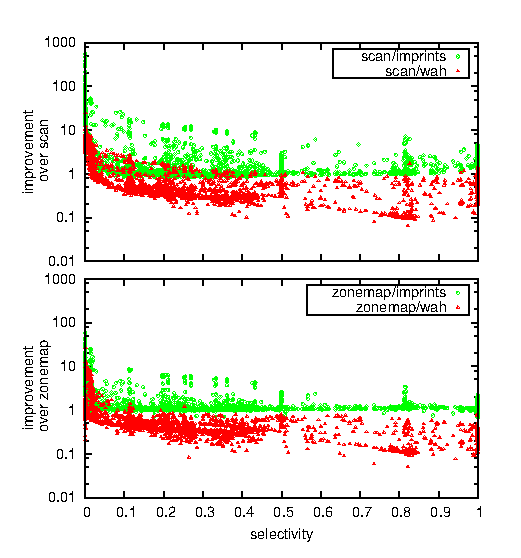
\includegraphics{figs/static/improv}
\caption{Factor of improvement over scan and zonemap.}
\label{fig:impr}
\end{figure}

We are interested in the factor of improvement that is achieved by
the imprints index over the sequential scan baseline and the competitive
zonemap indexing. Figure~\ref{fig:impr} depicts the factor of improvement
achieved for each query. A point above $1$ is translated as a factor of
improvement over the baseline, while a point below $1$ shows how many times
an approach is slower than the baseline. The upper graph of
Figure~\ref{fig:impr} shows with green circle points the improvement of
imprints over sequential scans, while the red triangles, the corresponding
improvement of bitmaps with WAH over sequential scans. Both imprints and WAH,
show a significant improvement for queries with high selectivity, i.e., when
less than 20\% of the tuples are returned. For imprints that improvement is in
some cases almost a $1000$ times faster, and for WAH over $10$. However, for
low selectivity queries, imprints become less competitive, while WAH can become
significantly slower than scans. This observation is aligned with the strategy
of most modern database systems, where, if the cost model of the query
optimizer detects a low selectivity selection, a sequential scan is preferred
over any index probing. Moreover, WAH is punished in a main memory setting. The
processing overhead of the WAH compression outweighs the throughput of data
that is achieved from main memory to the cpu cache. Therefore, WAH is more
suitable for cases where data do not reside in memory, but need to be fetched
from disk. Similarly, the bottom graph of Figure~\ref{fig:impr} depicts the
same comparison, but with zonemap indexing being the baseline, instead of
sequential scans. The same trend can be seen here, although zonemaps is more
competitive and thus the improvement factor for imprints is closer to $100$
times. However, in a few cases of low selectivity zonemaps can become faster
than imprints due to less computation needs.

\begin{figure}
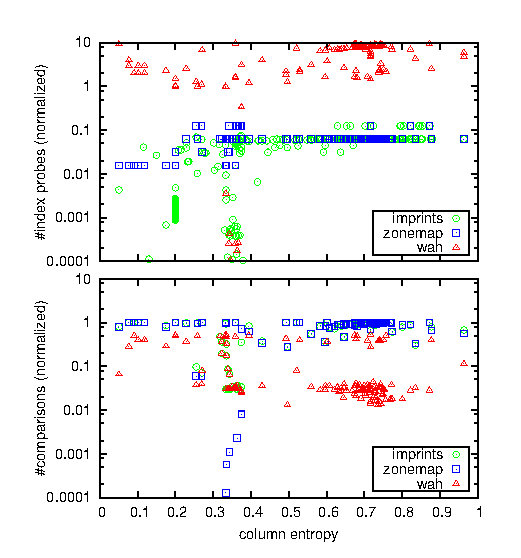
\includegraphics{figs/static/stats}
\caption{Number of index probes and value comparisons for queries with selectivity between $0.4$ and $0.5$.}
\label{fig:stats}
\end{figure}

Finally, we compare the number of index probes and data comparisons performed (originating from testing for false positives) normalized over the number of
records in a column. This experiment reveals implementation-independent
statistics for column imprints in comparison with zonemaps and WAH. The top
graph of Figure~\ref{fig:stats} shows the number of index probes, while the
bottom the number of comparisons, for all queries with selectivity between
$0.4$ and $0.5$. The number of index probes for WAH is the highest of all
indexes, almost always more than the number of total records. This is true
since for each record many bit vectors have to be probed. However, WAH achieves
the best filtering since the number of data comparisons is usually very low. On
the other hand, zonemaps have a steady number of index probes, i.e., exactly
the number of cachelines of the column. The number of comparisons for zonemaps
depends on the data skew and can vary. Column imprints achieve a balance
between index probes and data comparisons. Columns with high entropy entail
more index probes but less data comparisons. On the
other hand, columns with low entropy will need less index probes but more data
comparisons.

In conclusion, for high selectivity queries column imprints index can achieve a
factor of $1000$ improvement over sequential scans, and a factor of $100$ over
zonemap. Further experimentation, revealed that there is a correlation between
the query evaluation time and the sizes of the column, or the size of the
index, which in turn is correlated with the column entropy. We do not show
these graphs since they do not reveal any new insights into the performance of
imprints compared to zonemap or WAH index.
